\section*{CHƯƠNG 3. THIẾT KẾ HỆ THỐNG}
    \addcontentsline{toc}{section}{\numberline{}CHƯƠNG 3. PHƯƠNG PHÁP LUẬN}
    
\setcounter{section}{3}
    \setcounter{subsection}{0}
        \setcounter{figure}{0}
            \setcounter{table}{0}
%%-------------------------------------------------------%%
% --------------------------------------------------------%
%---------------------------------------------------------%

\subsection{Phân tích yêu cầu hệ thống}


\begin{figure}[!ht]
    \centering
    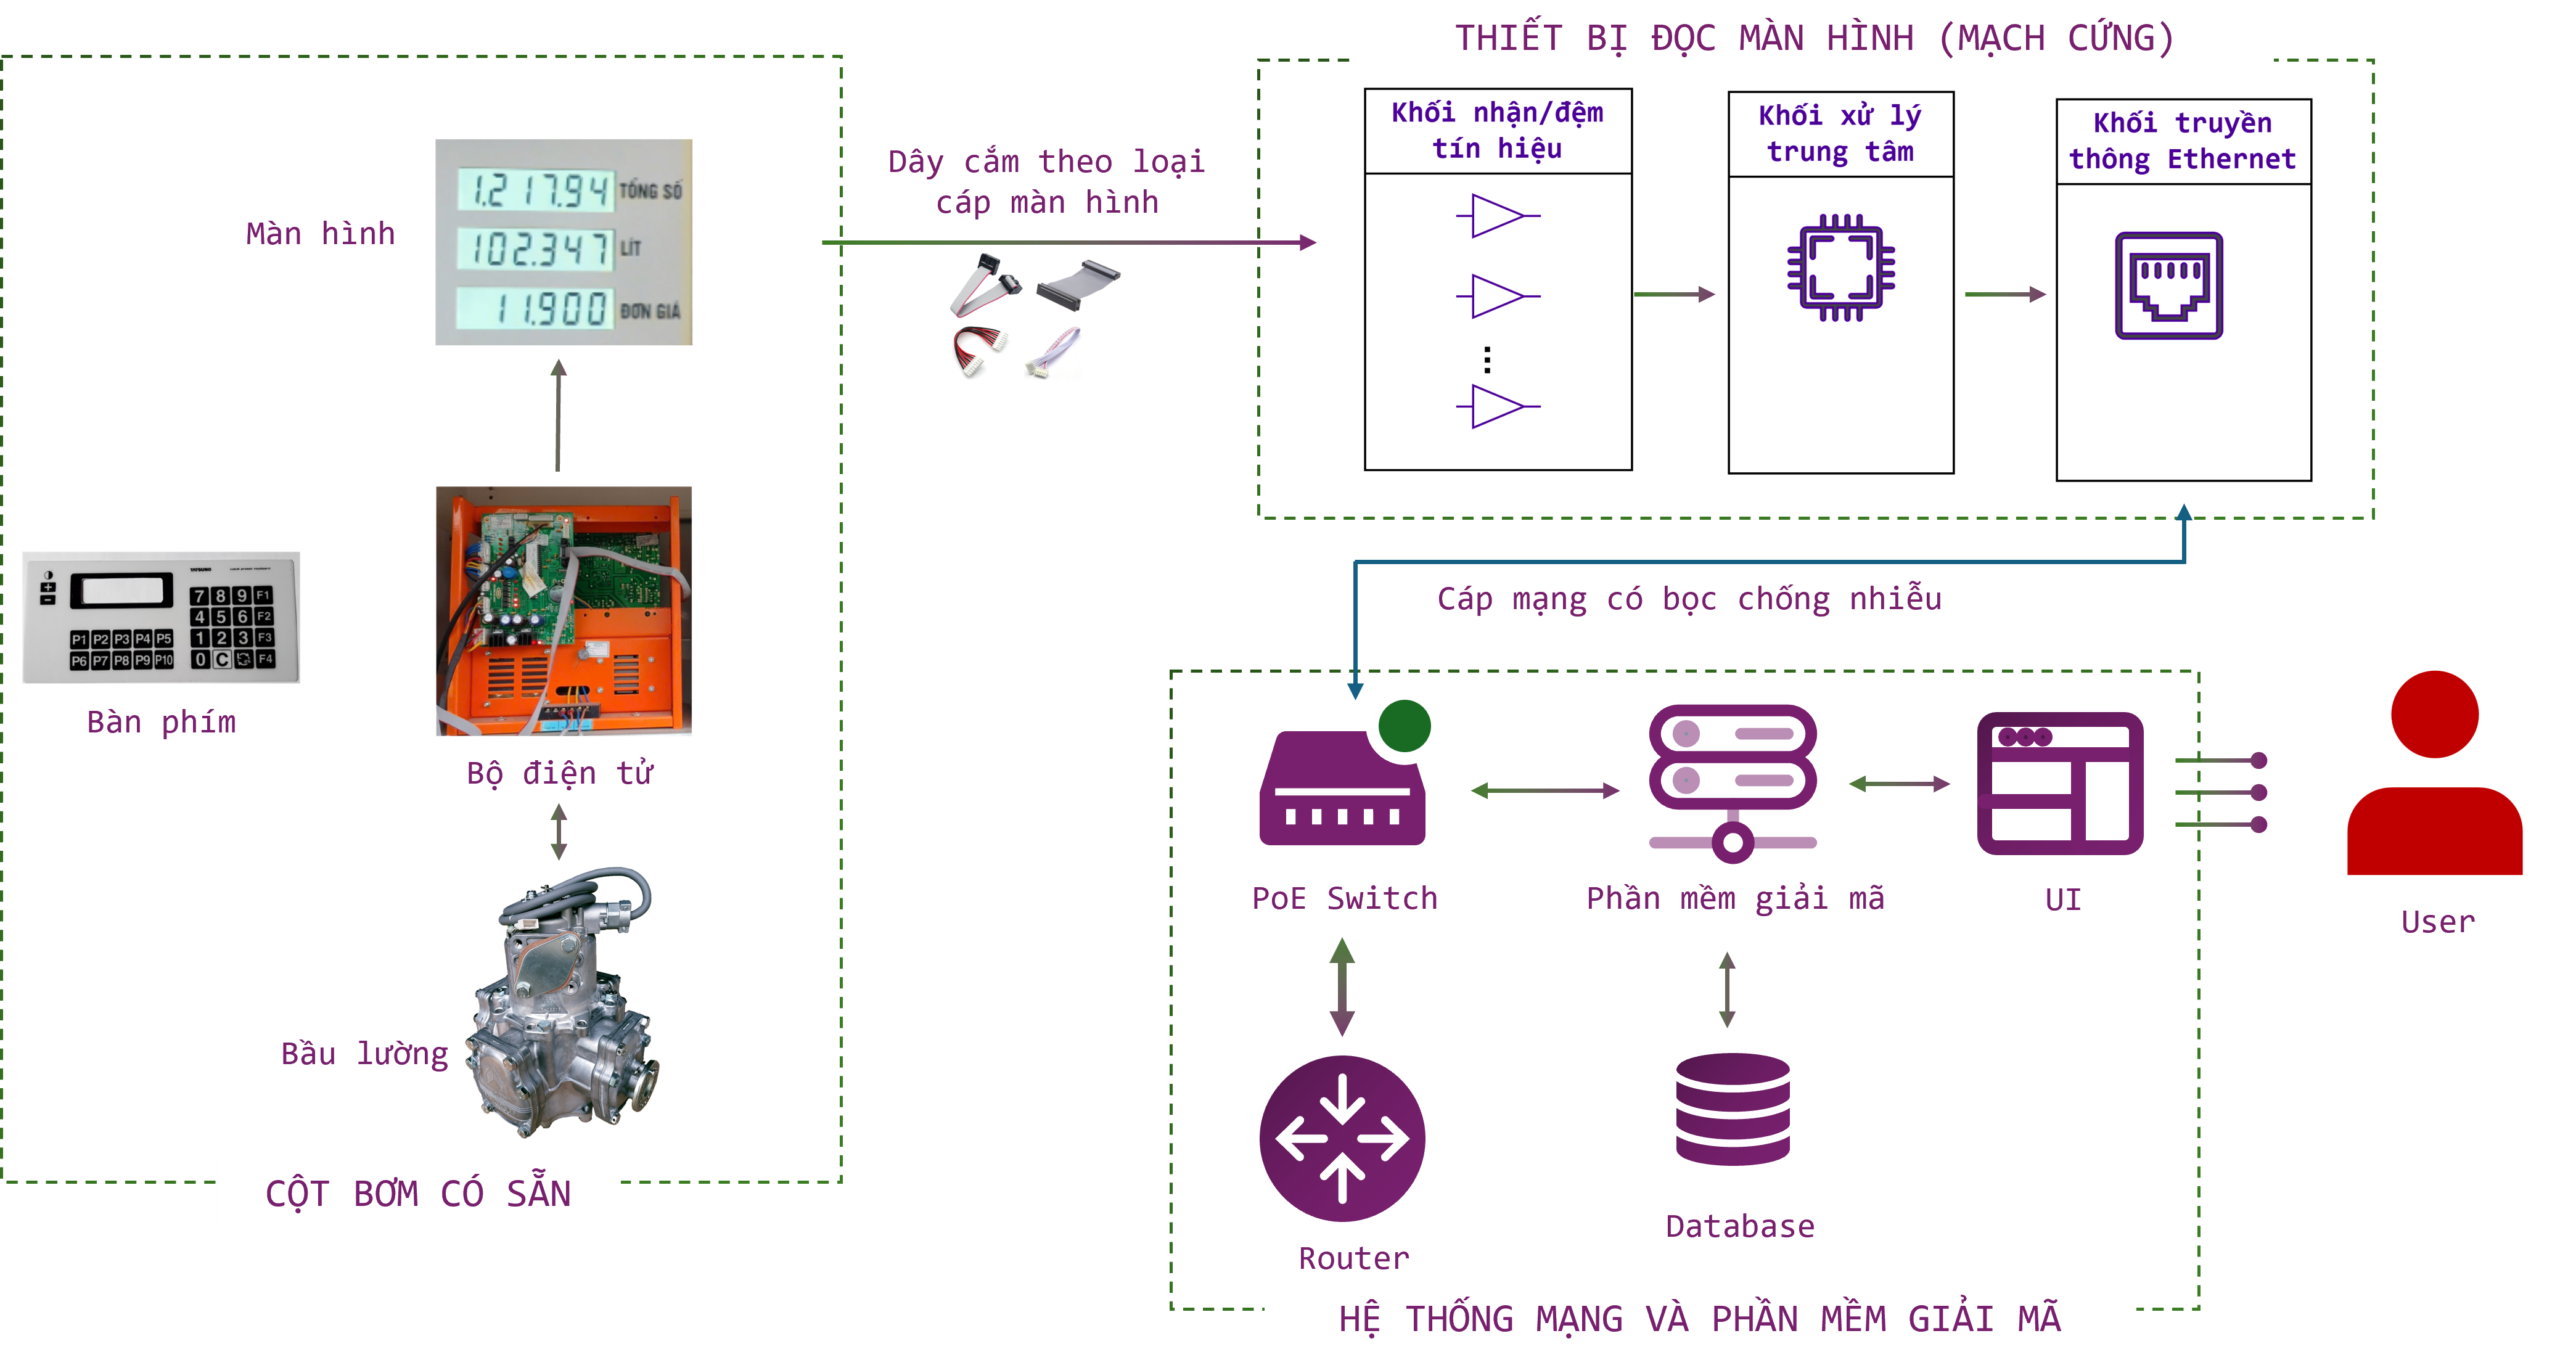
\includegraphics[width=1.0\linewidth]{Figures/Chap3_FunctionBlock-implementation.png}
    \caption{Các thành phần của hệ thống}
    \label{fig:hinh3.1}
\end{figure}

Các thành phần chính của hệ thống bao gồm:

\subsubsection{Thiết bị đọc ghi màn hình}


Là mạch cứng gắn vào màn hình cột bơm, thu dữ liệu thô màn hình:
\begin{itemize}
   
    \item Kích cỡ: vừa, có thể lắp đặt trong cột bơm
    \item Tần số lấy mẫu: 100Hz
    \item Cấp nguồn riêng
    \item Nguồn và tín hiệu vào được cách ly quang, đảm bảo không có tín hiệu quay ngược trở lại màn hình
    \item Có 2 relay đóng ngắt có thể nối nối tiếp với cột bơm
    \item Giao tiếp, gửi dữ liệu thông qua Ethernet
    \item (Optional) Đầu vào tín hiệu (cáp và bộ chuyển đổi tín hiệu) có thể thích hợp với nhiều loại màn hình khác ngoài ZCheng để phục vụ thu thập và phân tích thêm các loại cột bơm khác.
    
\end{itemize}



\subsubsection{Phần mềm giải mã}

Phần mềm giải mã đặt trong máy tính nội bộ tại trạm:

\begin{itemize}
    \item Đọc và giải mã tín hiệu tới màn hình với tần số 100Hz.
    \item Giao diện phần mềm hiển thị màn hình đã giải mã theo thời gian thực
    \item Phát hiện, lưu trữ các phiên bơm. Giao diện hiển thị các phiên bơm đã lưu trữ.
    \item Điều khiển đóng ngắt relay.
    \item Có cơ chế cập nhật firmware (OTA) cho thiết bị.    
\end{itemize}

\subsubsection{Hệ thống mạng}

\begin{itemize}
    \item POE Switch cấp nguồn riêng cho thiết bị đọc ghi màn hình
    \item Router điều khiển mạng LAN, cấp phát IP cho thiết bị
    \item Các thiết bị (thiết bị đọc ghi màn hình và phần mềm giải mã trong máy tính nội bộ) có thể tự động dò tìm và kết nối với nhau.
\end{itemize}

\subsection{Mô hình thiết kế tổng thể}

Phần này nêu ra sơ đồ khối chức năng các thành phần hệ thống. Qua đó mô tả chức năng cụ thể của thành phần thông qua các khối, đồng thời mô tả cách các khối giao tiếp với nhau.

\subsubsection{Sơ đồ khối chức năng thiết bị đọc ghi màn hình (Device)}

\begin{figure}[!ht]
    \centering
    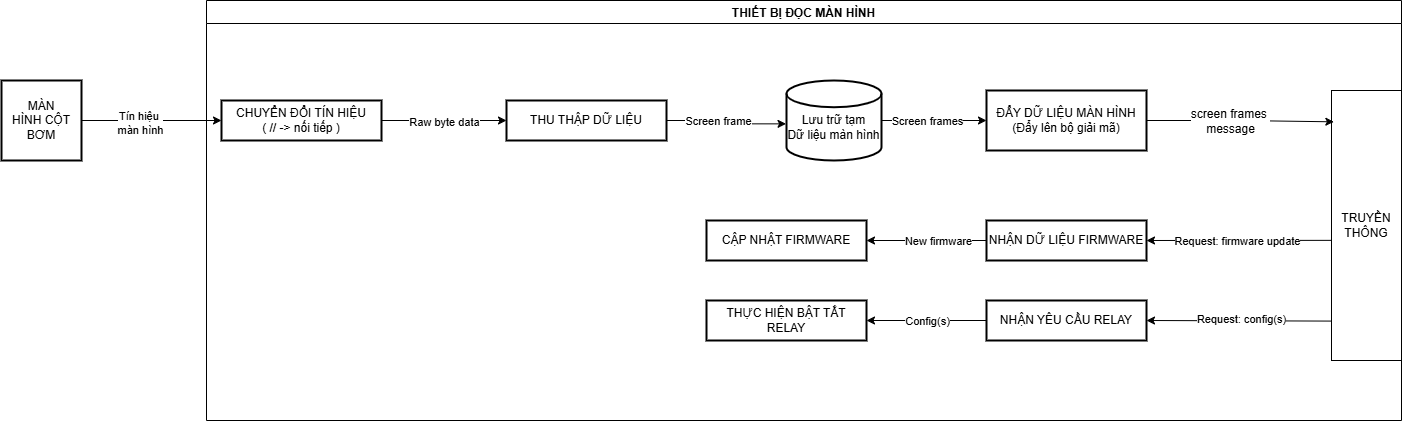
\includegraphics[width=1.0\linewidth]{Figures/Chap3_Device-FunctionBlock.png}
    \caption{Sơ đồ khối chức năng thiết bị đọc ghi màn hình (Device)}
    \label{fig:hinh3.2}
\end{figure}

\textbf{Giải thích các khối chức năng:} 

\begin{itemize}
    \item \textbf{Chuyển đối tín hiệu: }
    \subitem Nếu tín hiệu gửi tới màn hình cột bơm là nối tiếp, khối này đệm tín hiệu nối tiếp tới bộ Thu thập dữ liệu
    \subitem Nếu tín hiệu gửi tới màn hình cột bơm là song song, có nhiều chân dữ liệu, khối này chuyển đổi tín hiệu từ các chân thành tín hiệu nối tiếp -> các byte data để đệm tới bộ Thu thập dữ liệu.
    \item \textbf{Thu thập dữ liệu: } Thu thập các byte data tổng hợp thành các screen frame, lưu tạm vào 1 in-mem database.
    \item \textbf{Đẩy dữ liệu lên màn hình: } Thiết bị đọc màn hình tạo 1 message (request message) gồm nhiều screen frame để đẩy lên máy tính local
    \item \textbf{Nhận và cập nhật firmware mới: } Thiết bị đọc màn hình có thể nhận firmware mới từ máy tính local hoặc Logi Service và tự động cập nhật, khởi động lại
    \item \textbf{Nhận và cập nhật relay:} Thiết bị đọc ghi màn hình có thể nhận và thực hiện yêu cầu bật tắt relay 
    \item \textbf{Truyền thông:} Lấy địa chỉ IP, dò tìm địa chỉ của phần mềm giải mã và tự động kết nối. Truyền nhận dữ liệu với phần mềm giải mã thông qua mạng LAN.

\end{itemize}

\subsubsection{Sơ đồ khối chức năng phần mềm giải mã (Device Service)}

\begin{figure}[!ht]
    \centering
    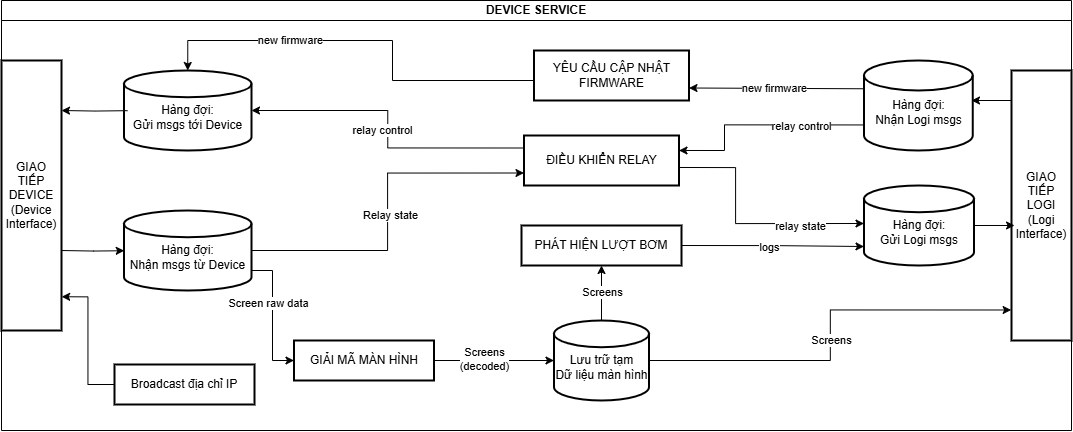
\includegraphics[width=1.0\linewidth]{Figures/Chap3_DeviceService-function-block.png}
    \caption{Sơ đồ khối chức năng phần mềm giải mã và chốt phiên bơm (Device Service)}
    \label{fig:hinh3.3}
\end{figure}




















